\chapter{Desarrollo}

\section{Map4rdf}
\subsection{Instalación}

Se ha optado por utilizar la máquina Virtual proporcionada en la Wiki del proyecto para minimizar la posibilidad
de incompatibilidades.

\section{GeoKettle}

Desde que se publicó ``A sustainable process and toolbox for geographical linked data generation and
publication: a case study with BTN100'' en 2019, GeoKettle ha dejado de estar soportado. La pagina oficial y de
documentación ya no están disponibles.
Un objetivo de este TFG es dar soporte GeoPackage a GeoKettle. No tiene sentido desarrollar soluciones de
``modernización'' sobre software abandonado.

Algunas funcionalidades de GeoKettle se integraron en PDI directamente y otras desaparecieron. 
Actualmente, el soporte GIS de Pentaho está dentro de PDI Spoon y además hay algunas funcionalidades más en
 el plugin llamado pentaho-gis-plugins\cite{gis-plugins}. Se actualizará la primera fase a:
\textbf{``replicar la funcionalidad y las transformaciones de GeoKettle + TripleGeo en la suite PDI.''}. 
Dado que se trata de replicar la funcionalidad anterior, se analizarán las tranformaciones realizadas por el OEG
en el repositorio de GitHub BTN100. Como se puede ver en la figura \ref{fig:spoon-missing-plugins}, partes del
workflow fallan. Es lo que se pretende solucionar.

\begin{figure}[H]
    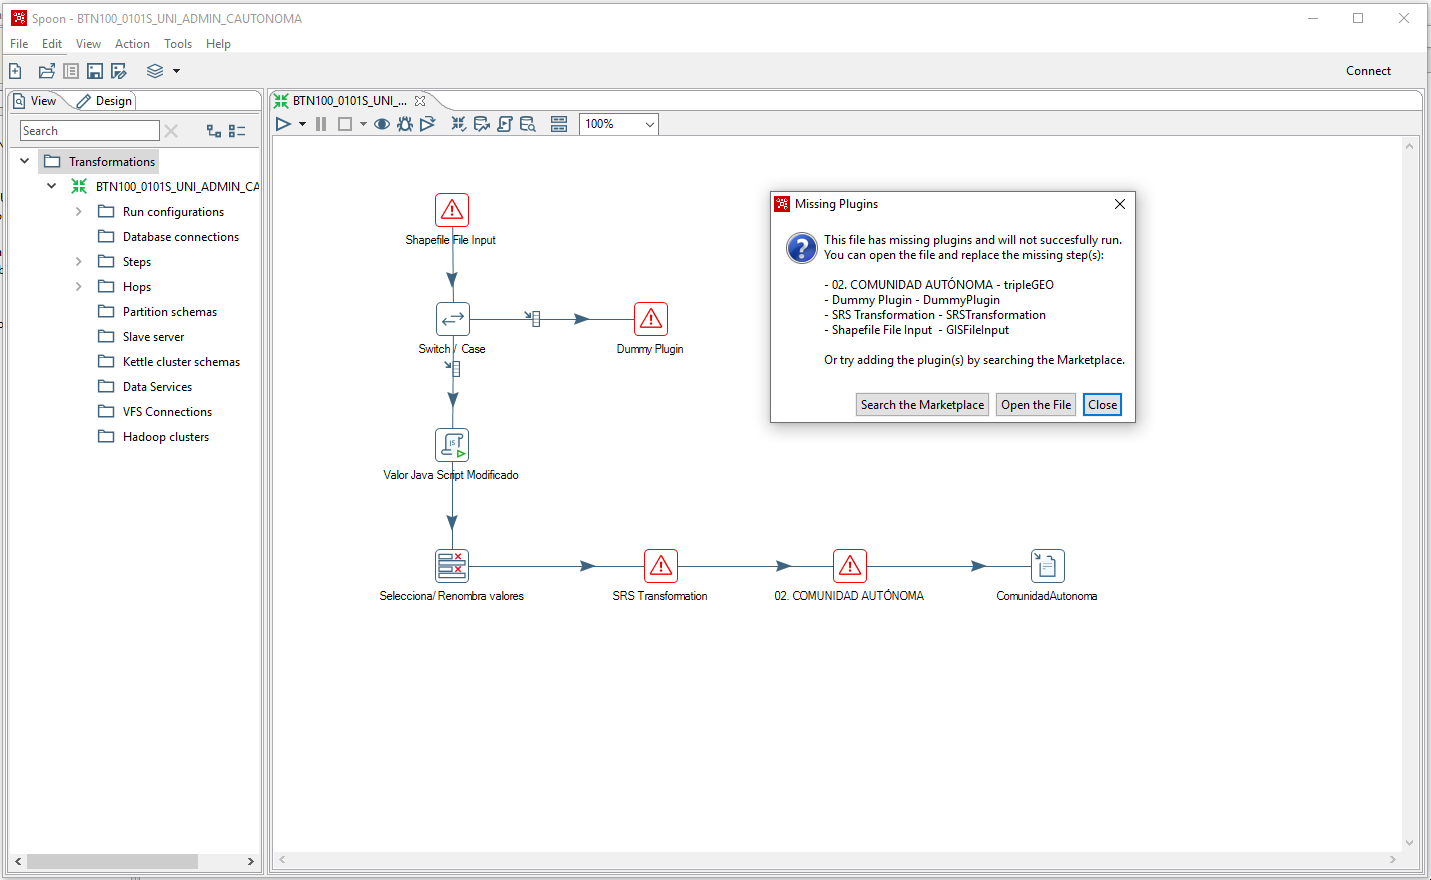
\includegraphics[width=\textwidth]{images/spoon-missing-plugins.png}
    \centering
    \caption{Workflow importado en la nueva suite}
    \label{fig:spoon-missing-plugins}
\end{figure}

\newpage
\subsection{Funcionamiento}

Para poder realizar el ``port'' de GeoKettle a Spoon, primero es necesario entender el funcionamiento y
transformaciones actuales de GeoKettle observando la entrada y salida de cada paso. Además esta manera se
observará mejor el flujo de datos y será más facil añadir soporte a GeoPackage en el futuro. No todas las
transformaciones tienen los mismos pasos, pero son parecidas. Como ejemplo se utilizarán los datos de
BTN100\_0101S\_UNI\_ADMIN y la transformación BTN100\_0101S\_UNI\_ADMIN\_CAUTONOMA. La transformación contiene
los siguientes pasos:

\begin{figure}[H]
    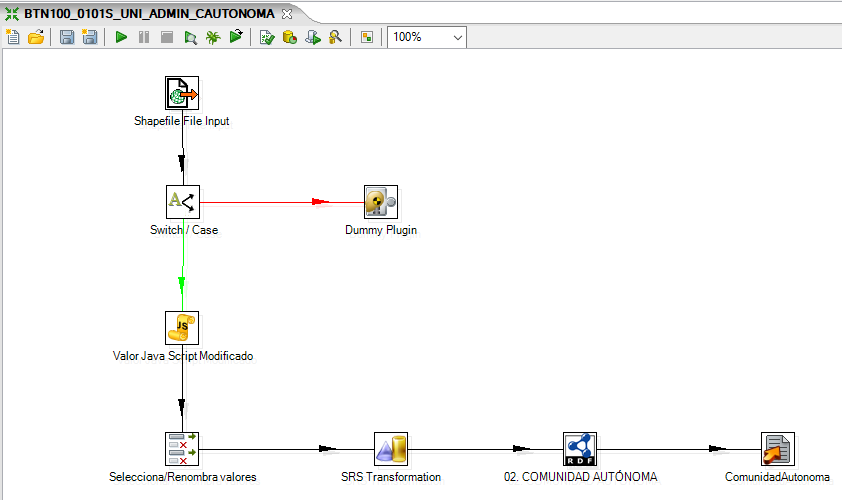
\includegraphics[width=\textwidth]{images/CCAA.png}
    \centering
    \caption{Transformación BTN100\_0101S\_UNI\_ADMIN\_CAUTONOMA}
    \label{fig:CCAA}
\end{figure}


\begin{enumerate}
    \item Shapefile File Input
    \item Switch Case
    \item Dummy Plugin
    \item Valor Java Script Modificado
    \item Selecciona/Renombra valores
    \item SRS Transformation
    \item TripleGeo
    \item Text Output
\end{enumerate}


\subsubsection{Shapefile File Input}

Lee el fichero shapefile.
\begin{enumerate}
    \item \textit{.shp}: Geometría fig.\ref{fig:shapefile}

        \begin{figure}[H]
            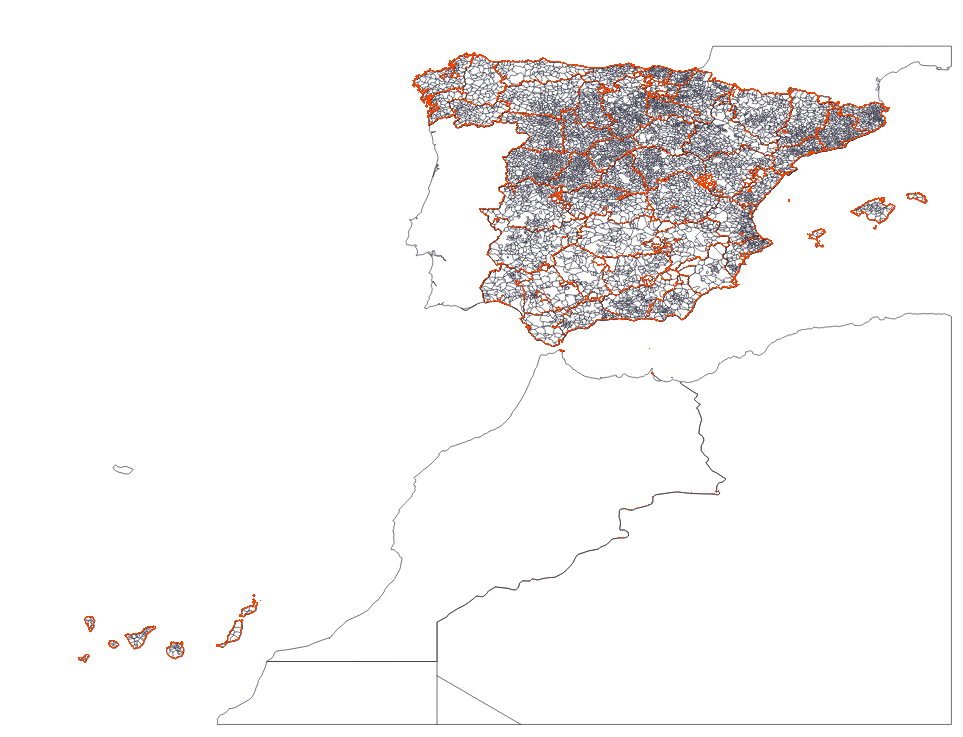
\includegraphics[width=0.7\textwidth]{images/shapefile.png}
            \centering
            \caption{Geometría contenida en el shapefile}
            \label{fig:shapefile}
        \end{figure}

    \item \textit{.dbf}: Datos asociados en columnas fig.\ref{fig:dbf}

        \begin{figure}[H]
            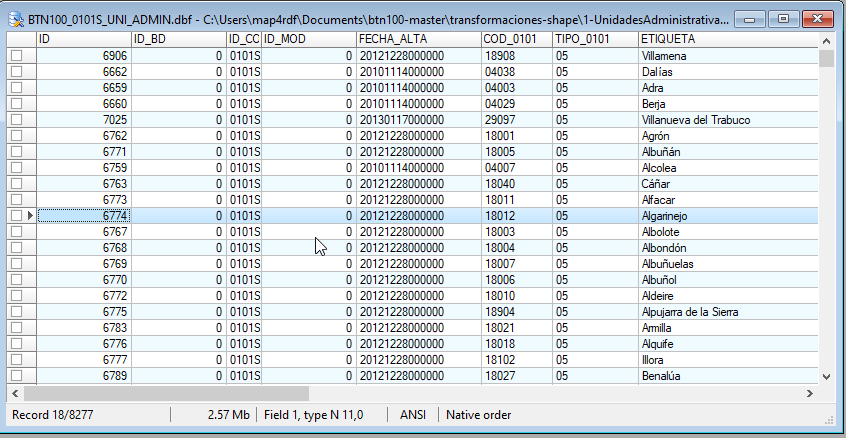
\includegraphics[width=0.7\textwidth]{images/dbf.png}
            \centering
            \caption{Datos columnares dbf asociados a la geometría}
            \label{fig:dbf}
        \end{figure}

    \item \textit{.shx}: Índice para acelerar búsquedas
    \item \textit{.prj}: Sistema de coordenadas
\end{enumerate}

\subsubsection{Switch case}
El switch case se encarga de filtrar y seleccionar las comunidades autónomas, identificadas por el valor 02 del
Campo TIPO\_0101. Si son una CCAA, se envían al paso 4, e.o.c. se envían al paso 3. fig.\ref{fig:switch} y
\ref{fig:tipo02}

\begin{figure}[H]
    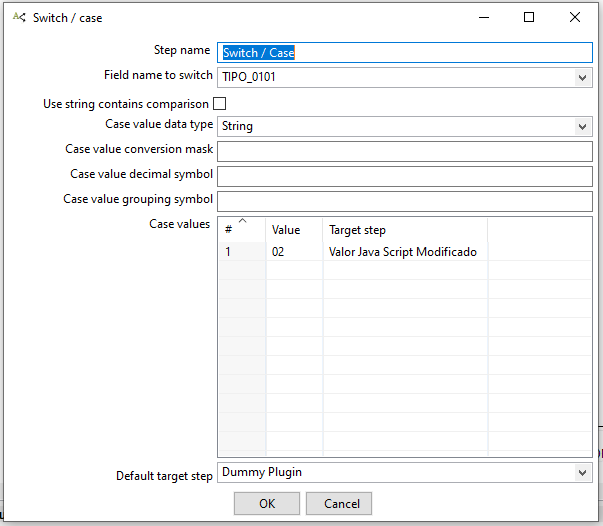
\includegraphics[width=0.7\textwidth]{images/switch.png}
    \centering
    \caption{Paso switch}
    \label{fig:switch}
\end{figure}

\begin{figure}[H]
    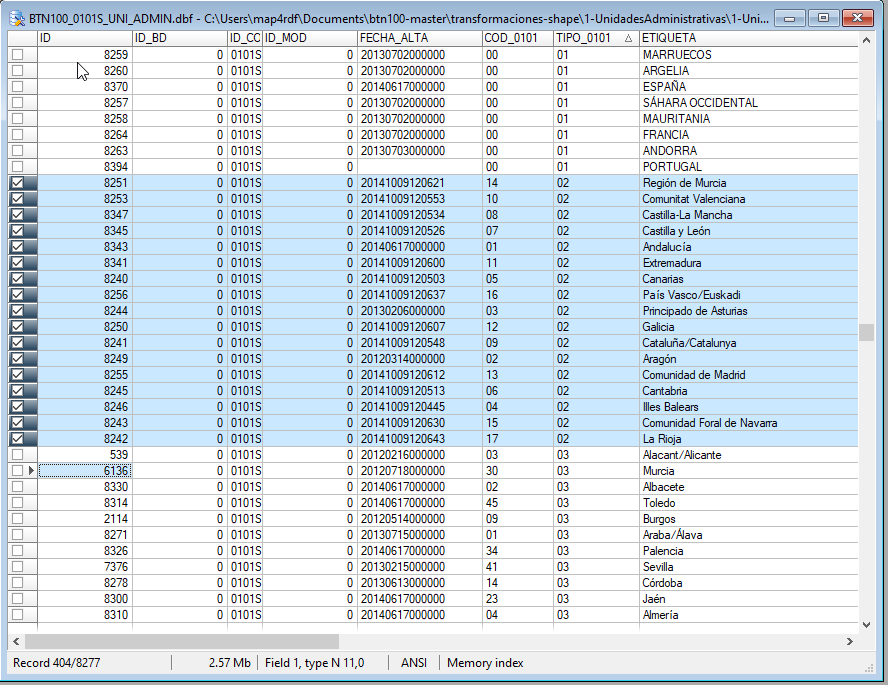
\includegraphics[width=\textwidth]{images/tipo02.png}
    \centering
    \caption{La filas correspondientes a las CCAA}
    \label{fig:tipo02}
\end{figure}

\subsubsection{Dummy Plugin}
No hace ninguna transformación, su propósito es recoger los datos innecesarios del switch.

\subsubsection{Valor Java Script Modificado}
El script cambia el formato de la fecha para facilitar la lectura: de YYYYMMDDHHMMSS a YYYY-MM-DD. También
crea un nuevo campo llamado identificador a partir del campo etiqueta, cambiando espacios por barras bajas, mayúsculas
por minúsculas, quitando tildes y signos de puntuación. fig.\ref{fig:script} y \ref{fig:fecha}

\begin{figure}[H]
    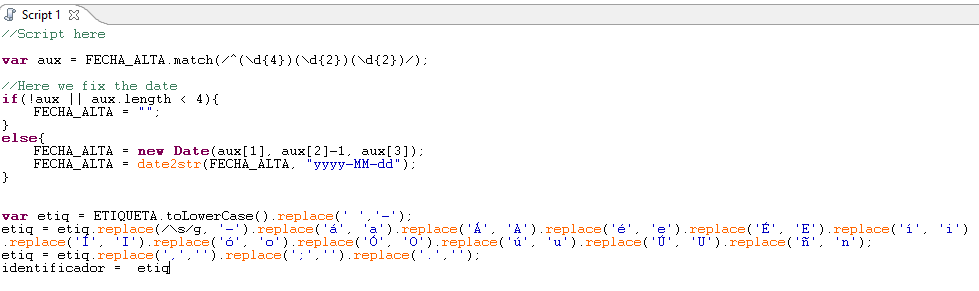
\includegraphics[width=\textwidth]{images/script.png}
    \centering
    \caption{Script Javascript}
    \label{fig:script}
\end{figure}

\begin{figure}[H]
    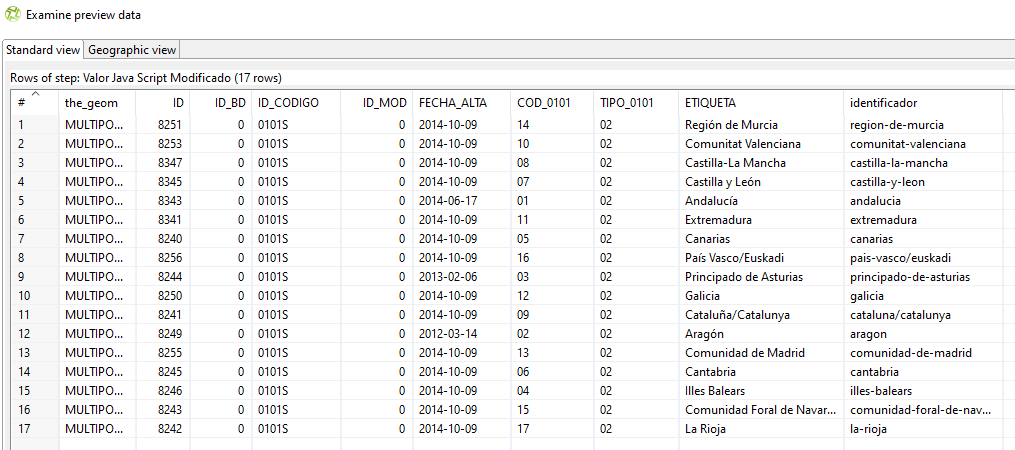
\includegraphics[width=\textwidth]{images/fecha.png}
    \centering
    \caption{Resultado del cambio de formato de fecha}
    \label{fig:fecha}
\end{figure}

\subsubsection{Selecciona/Renombra valores}
Cambia los metadatos de la columna FECHA\_ALTA para que sea reconocida como fecha. fig.\ref{fig:selecciona-renombra}

\begin{figure}[H]
    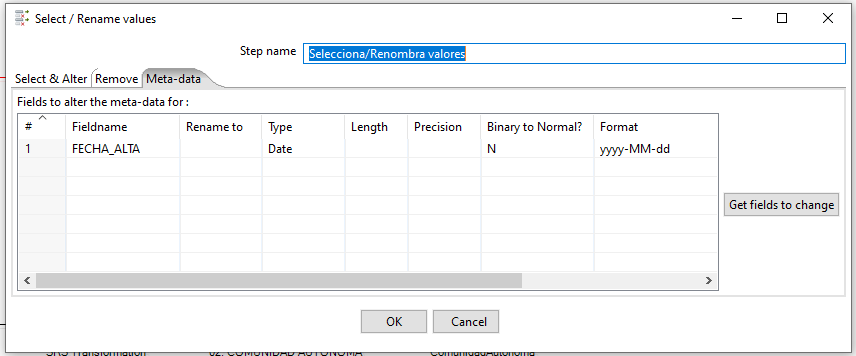
\includegraphics[width=\textwidth]{images/selecciona-renombra.png}
    \centering
    \caption{Selecciona/renombra valores}
    \label{fig:selecciona-renombra}
\end{figure}

\subsubsection{SRS Transformation}
Realiza la reproyección del sistema de coordenadas, en este caso de ETRS89 a WGS84. fig.\ref{fig:SRS}

\begin{figure}[H]
    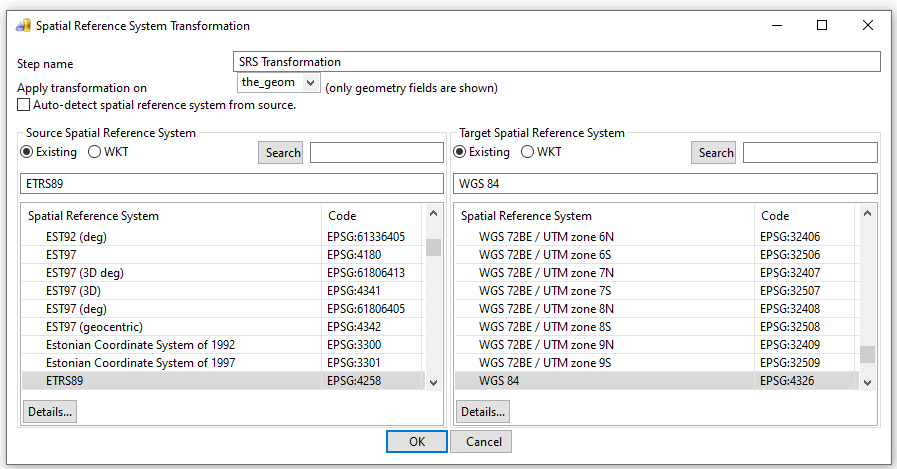
\includegraphics[width=\textwidth]{images/SRS.png}
    \centering
    \caption{Transformacion SRS}
    \label{fig:SRS}
\end{figure}

\subsubsection{TripleGeoKettle}
Transforma el shapefile del paso anterior en RDF en formato ttl. Se pueden configurar los parámetros asociados a la
ontologia y decidir si se muestran ciertas columnas o no. fig.\ref{fig:tripleGeoKettle}


\begin{figure}[H]
    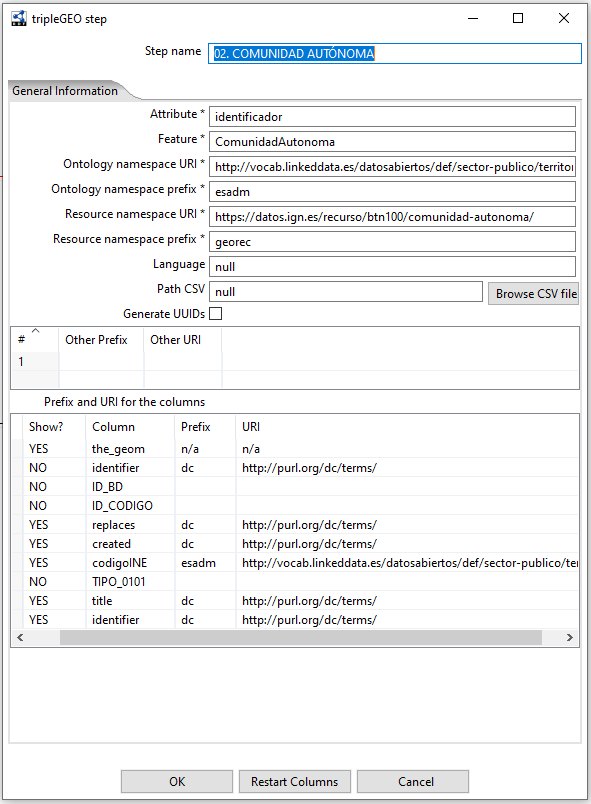
\includegraphics[width=0.9\textwidth]{images/tripleGeoKettle.png}
    \centering
    \caption{tripleGeoKettle}
    \label{fig:tripleGeoKettle}
\end{figure}

\subsubsection{Text file output}
Escribe los datos RDF en un fichero de texto con formato .ttl. fig.\ref{fig:text-file-output}
\begin{figure}[H]
    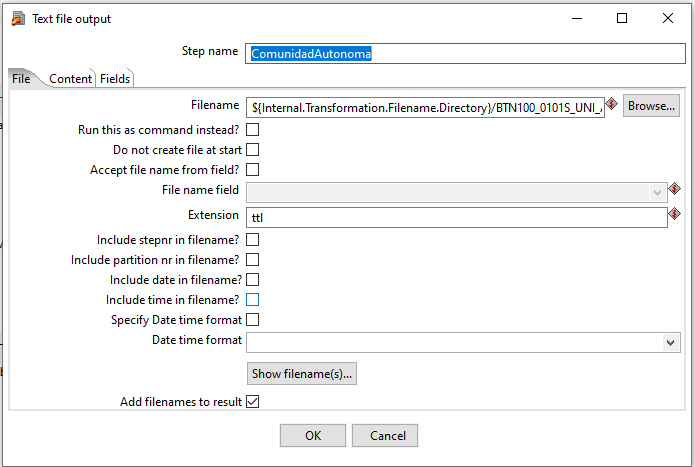
\includegraphics[width=\textwidth]{images/text-file-output.png}
    \centering
    \caption{text-file-output}
    \label{fig:text-file-output}
\end{figure}

\subsubsection{Resultado de la transformación}
\footnotesize
\begin{verbatim}
@prefix geo:   <http://www.w3.org/2003/01/geo/wgs84_pos#> .
@prefix geosparql: <http://www.opengis.net/ont/geosparql#> .
@prefix sf:    <http://www.opengis.net/ont/sf#> .
@prefix rdf:   <http://www.w3.org/1999/02/22-rdf-syntax-ns#> .
@prefix owl:   <http://www.w3.org/2002/07/owl#> .
@prefix xsd:   <http://www.w3.org/2001/XMLSchema#> .
@prefix georec: <https://datos.ign.es/recurso/btn100/comunidad-autonoma/> .
@prefix esadm: <http://vocab.linkeddata.es/datosabiertos/def/sector-publico/territorio#> .
@prefix rdfs:  <http://www.w3.org/2000/01/rdf-schema#> .
@prefix foaf:  <http://xmlns.com/foaf/0.1/> .
@prefix dc:    <http://purl.org/dc/terms/> .

georec:comunidad-de-madrid
        a                      esadm:ComunidadAutonoma ;
        rdfs:label             "comunidad-de-madrid" ;
        dc:created             "2014-10-09"^^xsd:date ;
        dc:identifier          "comunidad-de-madrid" ;
        dc:title               "Comunidad de Madrid" ;
        esadm:codigoINE        "13"^^xsd:int ;
        geosparql:hasGeometry  <https://datos.ign.es/recurso/btn100/comunidad-autonoma/...

georec:region-de-murcia
        a                      esadm:ComunidadAutonoma ;
        rdfs:label             "region-de-murcia" ;
        dc:created             "2014-10-09"^^xsd:date ;
        dc:identifier          "region-de-murcia" ;
        dc:title               "Región de Murcia" ;
        esadm:codigoINE        "14"^^xsd:int ;
        geosparql:hasGeometry  <https://datos.ign.es/recurso/btn100/comunidad-autonoma/...

<https://datos.ign.es/recurso/btn100/comunidad-autonoma/aragon/geometry>
        a                sf:Polygon ;
        geosparql:asWKT  "POLYGON ((-1.6174492000010632 40.94373283914169, -1.62366030000...
        ...
\end{verbatim}
\normalsize


\section{Port a PDI9}

\subsection{Tests con pentaho-gis-plugins}

El 3 de Marzo el plugin añadió soporte para el formato GeoPackage. Con el siguiente test se comprueba que los
componentes que se utilizarán para reemplazar las transformaciones antiguas funcionan correctamente.

\begin{figure}[H]
    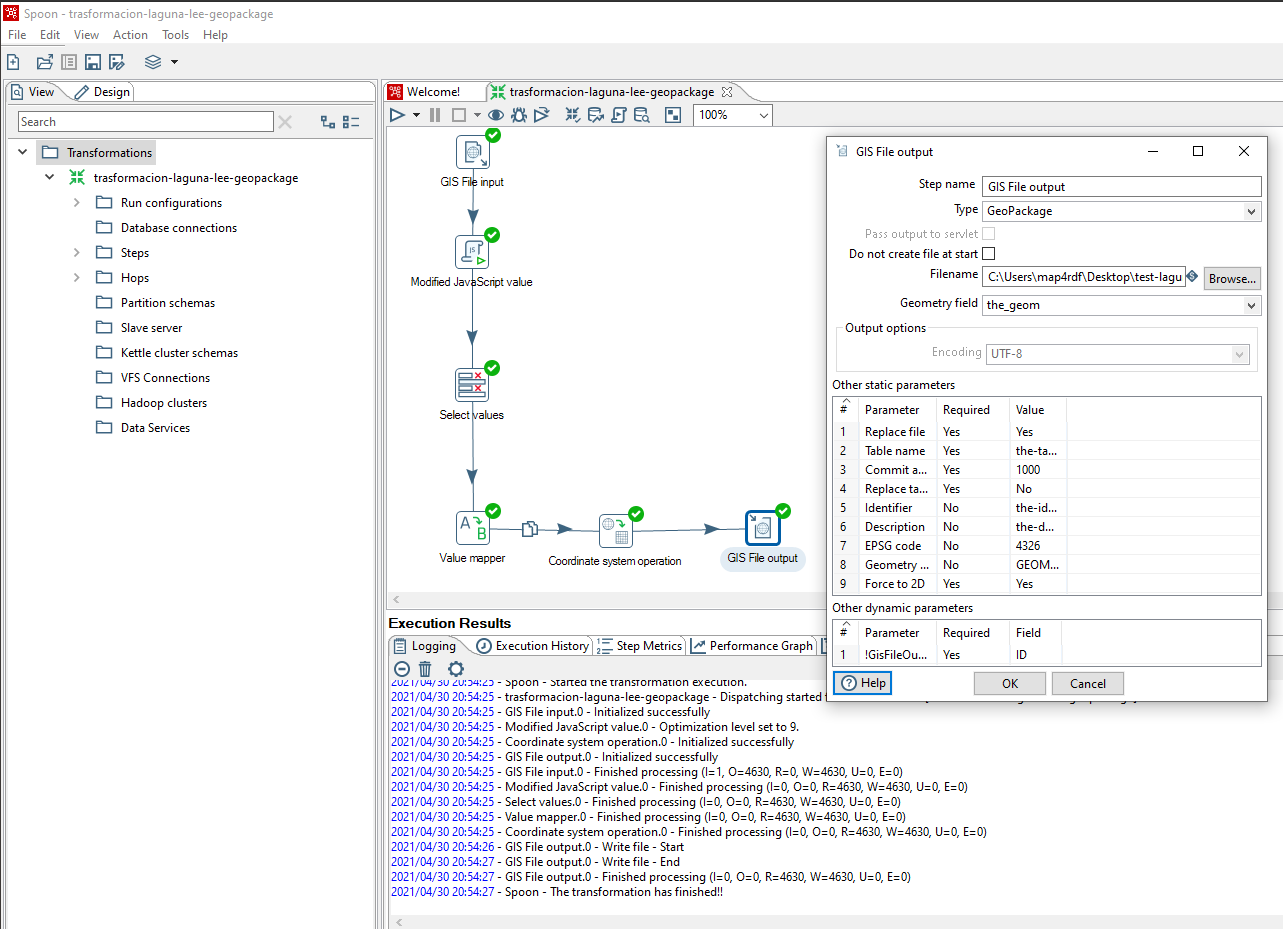
\includegraphics[width=\textwidth]{images/test-laguna-geopackage.png}
    \centering
    \caption{test-laguna-geopackage}
    \label{fig:test-laguna-geopackage}
\end{figure}

\subsection{Entorno de desarrollo}

\subsubsection{Dependencias e instalación}

En los ultimos años Pentaho ha pasado de utilizar Apache Ant a utilizar Apache Maven. TripleGeoKettle también
utilizaba Ant, y se ha decidido utilizar Maven por las ventajas que ofrece. El proyecto TripleGeoKettle contenía
una carpeta lib en la que se encontraban los .jar con las dependencias necesarias. Ahora, las dependencias se
administran con Maven y el pom.xml. Se incluyen los repositorios de Pentaho y OSGeo y las dependencias que se
quieren incluir. Las properties funcionan a modo de ``variable'' para poder cambiar la versión de pdi fácilmente
en un solo lugar.


\lstinputlisting[language=XML]{../TripleGeoKettle-PDI9/pom.xml}

A continuación se muestran los pasos para configurar el entorno de desarrollo en Arch Linux:

\begin{lstlisting}
# Instalar PDI desde AUR (los mirrors son mas rapidos que los de SourceForge)
yay -S pdi-ce
# Instalar Java 8
sudo pacman -S jdk8-openjdk
# Cambiar la version de java con
sudo archlinux-java set java-8-openjdk
# Instalar el Plugin de desarrollo
https://sourceforge.net/projects/pentaho/files/Pentaho%209.1/plugins/kettle-sdk-plugin-assembly-9.1.0.0-324.zip/download
# Instalar Maven
sudo pacman -S maven
# Descargar el settings.xml del repositorio de github en ~/.m2
https://raw.githubusercontent.com/pentaho/maven-parent-poms/master/maven-support-files/settings.xml
# Desde el directorio del plugin compilar y empaquetar el plugin
mvn clean package
# Instalarlo en PDI9 copiando el contenido del .zip generado en el directorio target
sudo cp target/tripleGeoKettle-oeg-1.jar /opt/pdi/plugins/steps/tripleGeoKettle-oeg-1/
\end{lstlisting}

\subsubsection{Pentaho sdk plugins}

Pentaho ofrece plugins\cite{pdi-sdk} muy sencillos de ejemplo que muestran cómo implementar un plugin. Para el port de
TripleGeoKettle se ha utilizado como referencia kettle-sdk-step-plugin que simplemente escribe Hello World. Con
él se ha probado la compilación, el pom.xml customizado, y pruebas varias como cambiar el icono o el nombre.


\section{Proceso de porteo}

Se comienza con el sdk de Pentaho y se realizan los cambios necesarios para integrar TripleGeoKettle en el nuevo
entorno. Se muestran las imagenes del antes y después de la estructura de carpetas. fig.\ref{fig:directorios-sdk}
y \ref{fig:directorios-TGK}

\begin{figure}[H]
    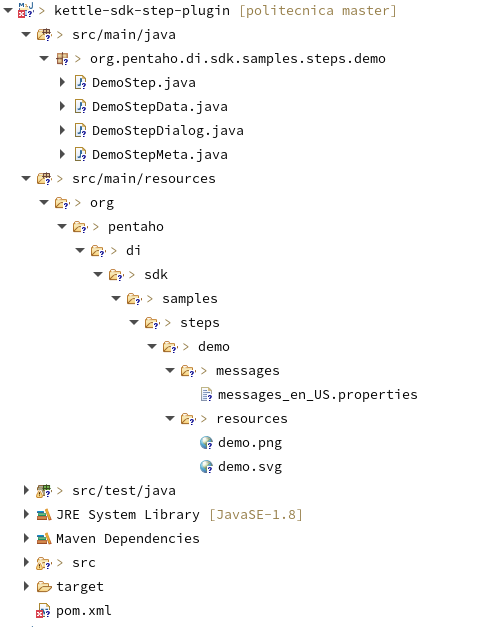
\includegraphics[width=0.7\textwidth]{images/directorios-sdk.png}
    \centering
    \caption{Estructura de carpetas del sdk}
    \label{fig:directorios-sdk}
\end{figure}

\begin{figure}[H]
    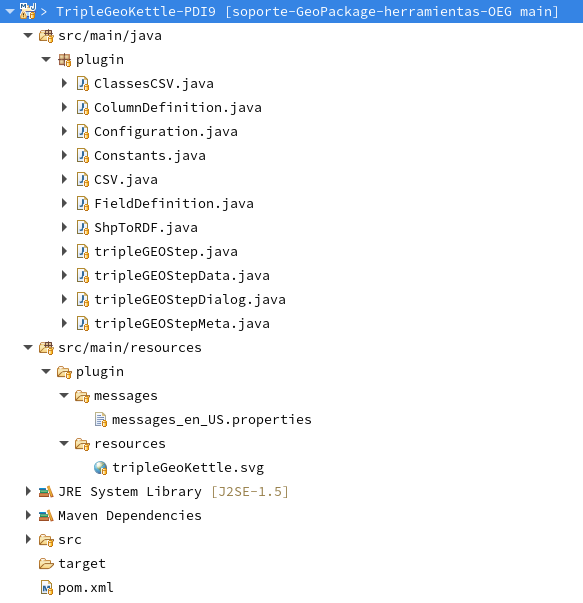
\includegraphics[width=0.7\textwidth]{images/directorios-TGK.png}
    \centering
    \caption{Estructura de carpetas de TripleGeoKettle portado}
    \label{fig:directorios-TGK}
\end{figure}

\textbf{Pasos seguidos:}

\begin{enumerate}
    \item Cambiar el nombre del paquete a ``plugin''. Es importante que el de java y el de resources tengan el
        mismo nombre para que los dialogos lean el fichero properties correctamente.

    \item Cambiar messages.properties
\begin{lstlisting}
#sdk properties
tripleGEO.FieldName.Label=Output field name
tripleGEO.CheckResult.ReceivingRows.OK=Step is receiving input from other steps.
tripleGEO.CheckResult.ReceivingRows.ERROR=No input received from other steps!

tripleGEOStep.Name=TripleGeoKettle
tripleGEOStep.TooltipDesc=An ETL Tool for Transforming Geospatial Data into RDF under the GeoSPARQL standard.
tripleGEOStep.DocumentationURL=https://github.com/oeg-upm/geo.linkeddata.es-TripleGeoKettle/wiki
tripleGEOStep.CasesURL=https://github.com/oeg-upm/geo.linkeddata.es-TripleGeoKettle/issues
tripleGEOStep.ForumURL=https://github.com/oeg-upm/geo.linkeddata.es-TripleGeoKettle/issues
tripleGEOStep.Linenr=Linenr {0}
tripleGEOStep.Error.NoOutputField=Could not find Output Field in row

# tripleGeoKettle custom properties
tripleGEOStepDialog.Shell.Title=tripleGEO step
tripleGEOStepDialog.Tab.MainTab=General Information
tripleGEOStepDialog.AttributeName.Label=Attribute *
tripleGEOStepDialog.Feature.Label=Feature *
tripleGEOStepDialog.OntologyNS.Label=Ontology namespace URI *
tripleGEOStepDialog.OntologyNSPrefix.Label=Ontology namespace prefix *
tripleGEOStepDialog.ResourceNS.Label=Resource namespace URI *
tripleGEOStepDialog.ResourceNSPrefix.Label=Resource namespace prefix *
tripleGEOStepDialog.Language.Label=Language
tripleGEOStepDialog.PathCSV.Label=Path CSV
tripleGEOStepDialog.PathCSVButton.Label=Browse CSV file
tripleGEOStepDialog.PathCSVButtonTooltip.Label=Browse for CVS file
tripleGEOStepDialog.uuids.Label=Generate UUIDs
tripleGEOStepDialog.Fields.Label=Other prefix and URI
tripleGEOStepDialog.other.Label=Other URI
tripleGEOStepDialog.otherPrefix.Label=Other Prefix
tripleGEOStepDialog.Column.Label=Column
tripleGEOStepDialog.Columns.Label=Prefix and URI for the columns
tripleGEOStepDialog.otherColumns.Label=URI
tripleGEOStepDialog.otherPrefixColumns.Label=Prefix
tripleGEOStepDialog.ShowColumns.Label=Show?
tripleGEOStepDialog.RestartFields.Button=Restart Columns
\end{lstlisting}

    \item Modificar la annotation @Step de DemoStepMeta.java. Se utiliza para que el programa reconozca y
        categorice el plugin correctamente.
\begin{lstlisting}
@Step(
   id = "TripleGeoKettle",
   name = "tripleGEOStep.Name",
   description = "tripleGEOStep.TooltipDesc",
   image = "plugin/resources/tripleGeoKettle.svg",
   categoryDescription = "i18n:org.pentaho.di.trans.step:BaseStep.Category.Transform",
   i18nPackageName = "tripleGeoKettle",
   documentationUrl = "tripleGEOStep.DocumentationURL",
   casesUrl = "tripleGEOStep.CasesURL",
   forumUrl = "tripleGEOStep.ForumURL"
   )
\end{lstlisting}

    \item Cambiar los nombres de las clases de Demo a TripleGeoKettle.
    \item Importar las clases java auxiliares de tripleGeoKettle.
    \item Hay un metodo deprecado en tripleGeoStepMeta.java: Valuemeta(). Se utiliza el constructor sin
        parámetros y luego se le asigna el tipo 2. Para sustituirlo, como el tipo es 2, que segun esta
        tabla\cite{tabla-string} significa string, es necesario cambiarlo a new ValueMetaString.

\item Error en los metodos readRep y saveRep, hay que importar ObjectId
 y cambiar long por ObjectId en la cabecera de la función.

\item Cambiar la siguiente línea para que la clase Dialog lea correctamente los contenidos del fichero properties.

\begin{lstlisting}
main/java/plugin/tripleGEOStepDialog.java
69: private static String PKG = tripleGEOStepDialog.class.getPackage().getName();
\end{lstlisting}

\item PDI9 utiliza iconos .svg y proporciona una guía de diseño\cite{guia-diseno}. Por tanto se ha actualizado el
    icono antiguo .png a .svg con los nuevos colores fig.\ref{fig:icono-TGK}
\end{enumerate}

\begin{figure}[H]
  \centering
    \includesvg{../TripleGeoKettle-PDI9/src/main/resources/plugin/resources/tripleGeoKettle.svg}
    \caption{Nuevo icono svg}
    \label{fig:icono-TGK}
    \centering
\end{figure}

\subsection{Resultado parcial}

La base del porteo se ha realizado correctamente como se puede ver en la figura \ref{fig:TGK-portado}. El dialogo
se abre y se pueden cambiar los parámetros de configuración. También es capaz de leer la salida del paso anterior
de SRS. Sin embargo, todavía no funciona correctamente. Probablemente se debe a que el paso
anterior (transformación de coordenadas) pasa su información de manera distinta al de GeoKettle (en PDI le llegan
9 campos y en GeoKettle 8). Será necesario seguir los pasos de la documentación para conectar el debugger y solucionar el
problema de NullPointerException.

\begin{figure}[H]
    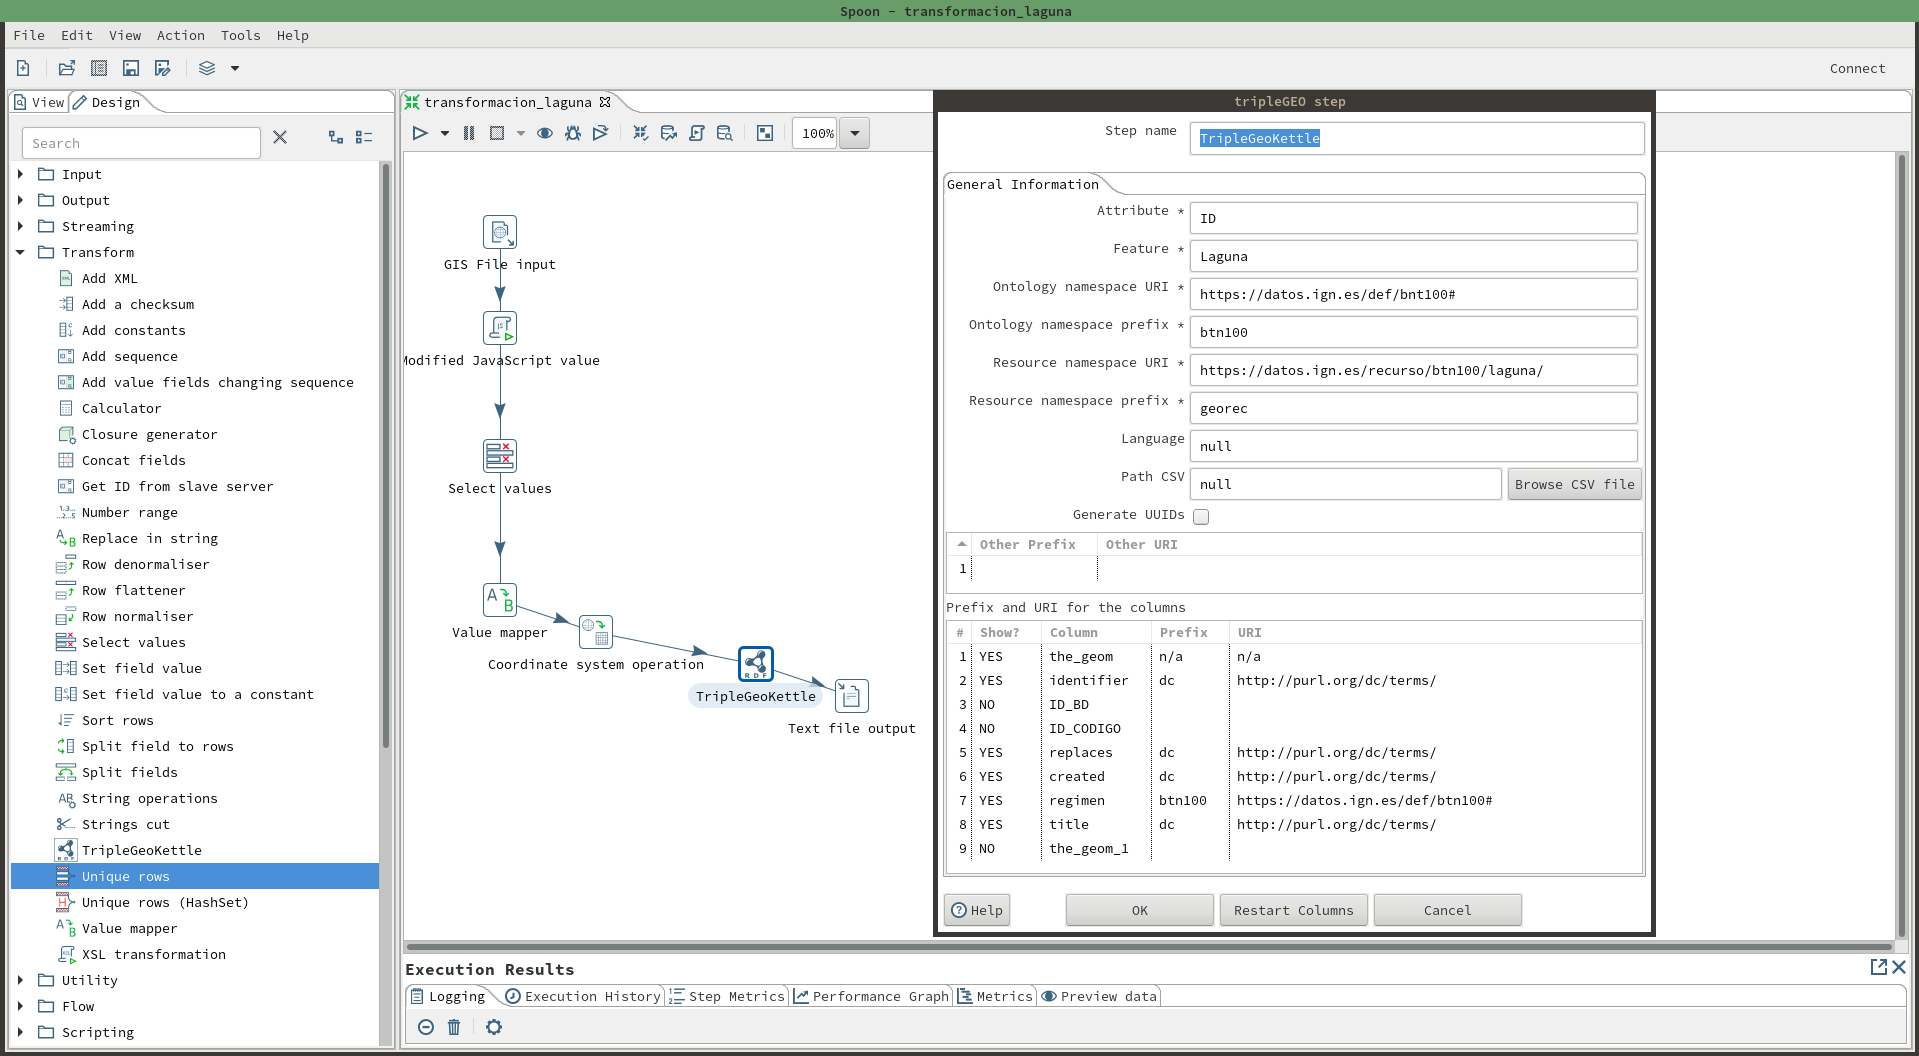
\includegraphics[width=\textwidth]{images/TGK-portado.png}
    \centering
    \caption{TripleGeoKettle corriendo en PDI9}
    \label{fig:TGK-portado}
\end{figure}

